\section{Anisotropic Filtering}
\frame{\sectionpage}

\begin{frame}{Principle}

\begin{itemize}
\item Iterative method
% \item Using knowledges about neighboors with derivation filters
\item \href{https://en.wikipedia.org/wiki/Partial_differential_equation}{PDE-based method}
\end{itemize}

\end{frame}

\begin{frame}{PDE meaning ?}
Partial Differential Equation (PDE): Differential equation with a function as solution
\end{frame}

\begin{frame}{Perona-Malik Model: Heat PDE}
\only<-2>{

\uncover<+->{

$\begin{cases}
I_{0} = I_\text{noisy} \\
I_{k+1} = I_{k} + \lambda [\sum\limits_{d \in Dir} 
(f_\text{diffusion} \circ (I_{k} \ast \nabla_{d}))] \\
\end{cases}$
}

\vspace{1cm}

\uncover<+->{
\begin{itemize}
\item $\lambda$ = hyper-parameter
\item $Dir = \left\lbrace \text{North}, \text{East}, \text{South}, \text{West} \right\rbrace$
\item $k$ = iteration number
\item $\nabla_{d}$ = derivation kernel with direction $d$
\item $f_\text{diffusion}$ = heat diffusion function
\end{itemize}
}

}

\end{frame}

\begin{frame}{Derivation kernels}
\begin{columns}

\column{.5\textwidth}
\centering
\begin{align*}
    \nabla_\text{North} = \begin{bmatrix} 0 & 1 & 0 \\ 0 & -1 & 0 \\ 0 & 0 & 0 \end{bmatrix}
\end{align*}
\begin{align*}
    \nabla_\text{South} = \begin{bmatrix} 0 & 0 & 0 \\ 0 & -1 & 0 \\ 0 & 1 & 0 \end{bmatrix}
\end{align*}

\column{.5\textwidth}
\centering
\begin{align*}
    \nabla_\text{West} = \begin{bmatrix} 0 & 0 & 0 \\ 1 & -1 & 0 \\ 0 & 0 & 0 \end{bmatrix}
\end{align*}
\begin{align*}
    \nabla_\text{Est} = \begin{bmatrix} 0 & 0 & 0 \\ 0 & -1 & 1 \\ 0 & 0 & 0 \end{bmatrix}
\end{align*}
\end{columns}

\end{frame}

\begin{frame}{Heat diffusion functions}

\only<-2>{

\uncover<+->{
$f_\text{diffusion} : \mathcal{R_{+}} \to \mathcal{R^{*}_{+}}$ such that
$\begin{cases}
f_\text{diffusion}(0) = 1 \\
\lim\limits_{u \to +\infty} f_\text{diffusion}(u) = 0
\end{cases}$
}

\vspace{1cm}
\uncover<+->{

Examples: \\

\begin{columns}

\column{.5\textwidth}
\centering
\begin{align*}
f_\text{diffusion}(u) = \frac{1}{1 + (\frac{u}{k})^{2}}
\end{align*}

\column{.5\textwidth}
\centering
\begin{align*}
f_\text{diffusion}(u) = e^{-(\frac{u}{k})^{2}}
\end{align*}

\end{columns}

\vspace{1cm}
with $k \in \mathcal{R^{*}_{+}}$
}
}

\end{frame}

\begin{frame}{Notation about $f_\text{diffusion} \circ (I_{k} \ast \nabla_{d})$}

Set $M = I_{k} \ast \nabla_{d}$.

\vspace{0.5cm}

\begin{align*}
f_\text{diffusion} \circ M
&= f_\text{diffusion} \circ \begin{bmatrix}
    m_{0, 0} & \dots & m_{0, M} \\
    \vdots & \ddots & \vdots \\
    m_{0, N} & \dots & m_{M, N}
\end{bmatrix} \\ 
&= \begin{bmatrix}
    f_\text{diffusion}(m_{0, 0}) & \dots & f_\text{diffusion}(m_{0, M}) \\
    \vdots & \ddots & \vdots \\
    f_\text{diffusion}(m_{0, N}) & \dots & f_\text{diffusion}(m_{M, N})
\end{bmatrix}
\end{align*}

\end{frame}

\begin{frame}{Algorithm}
\begin{algorithm}[H]
    \caption{Filtering Algorithm} % \label{euclid}
    \begin{algorithmic}[1]
        \Procedure{Denoising With Anisotropic Filter}{}\newline
        \textbf{Input:} $I$, $\lambda$, $N$ \\
        \textbf{Output:} $I_{N-1}$
        \State{$I_{0} = I$}
        \For{\texttt{$k \in [ 0, N [$}}
            \State{$I_{k+1} = I_{k} + \lambda [\sum\limits_{d \in Dir} 
(f_\text{diffusion} \circ (I_{k} \ast \nabla_{d}))]$}
        \EndFor
        \EndProcedure
    \end{algorithmic}
    % \label{alg_1}
\end{algorithm}
\end{frame}



% \begin{frame}{Results (with $N = 40$)}
% \centering
% \begin{columns}
% \column{.5\textwidth}
% \centering
% 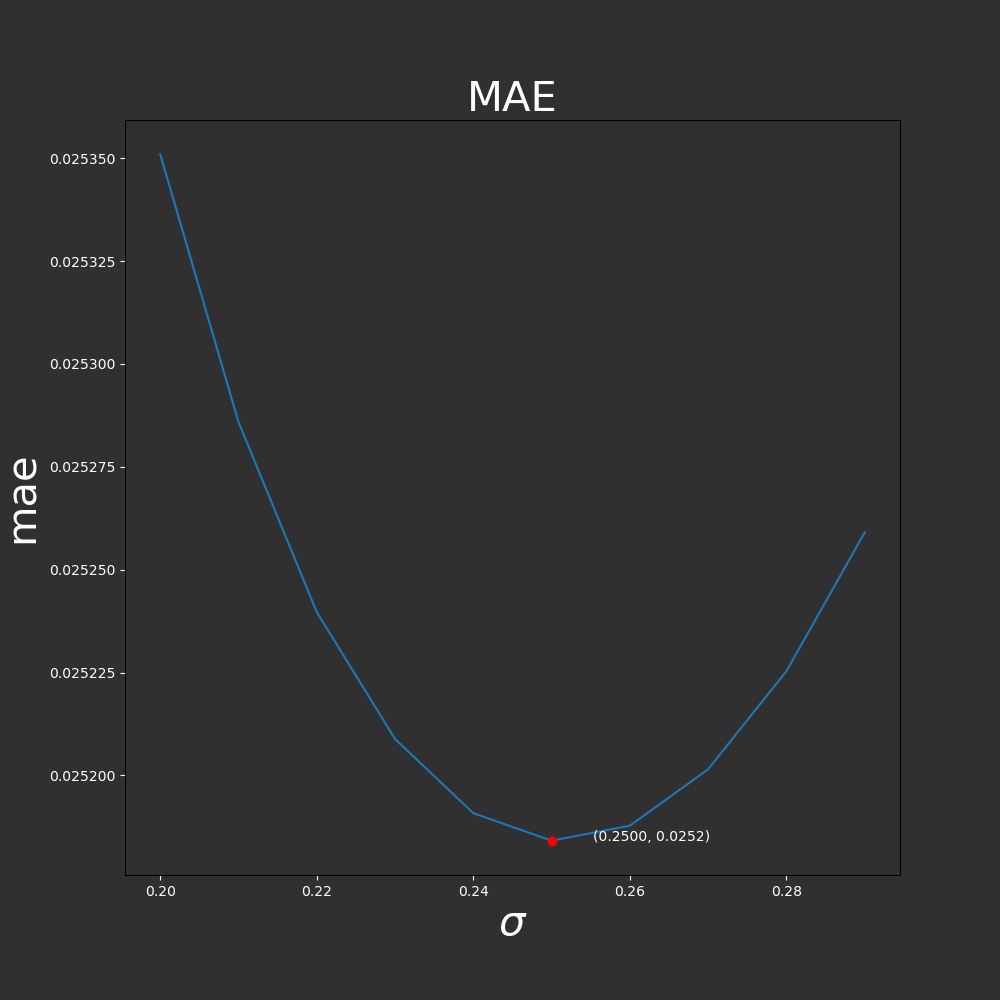
\includegraphics[scale=0.25]{results/anisotropic/plot_mae.jpg}
% \column{.5\textwidth}
% \centering
% 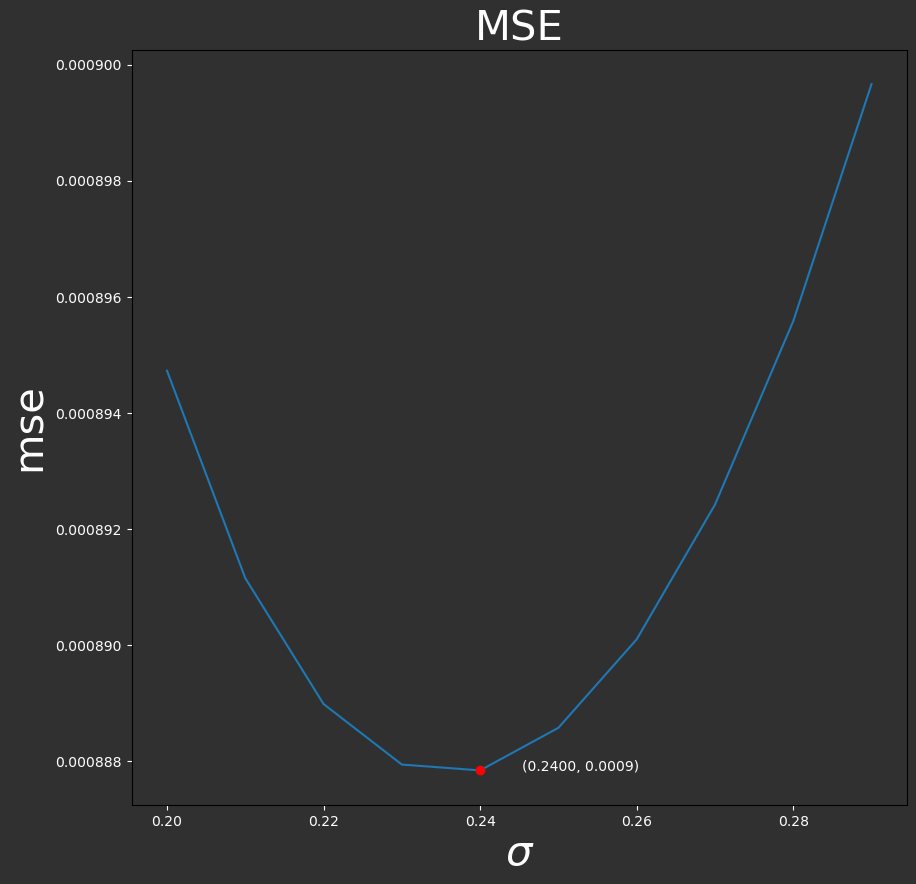
\includegraphics[scale=0.25]{results/anisotropic/plot_mse.jpg}
% \end{columns}
% \end{frame}

% \begin{frame}{Results (with $N = 40$)}
% \centering
% \begin{columns}
% \column{.5\textwidth}
% \centering
% 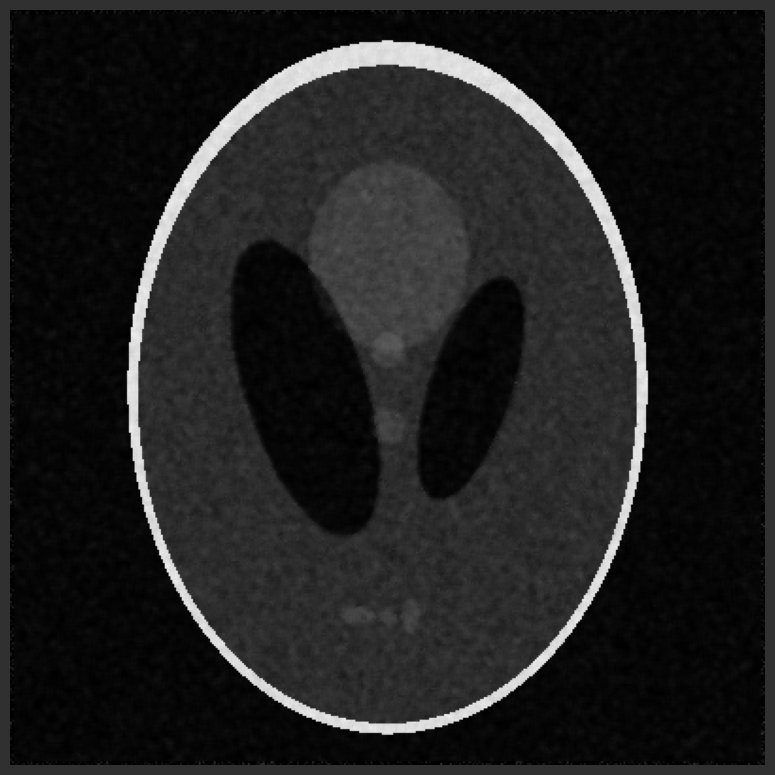
\includegraphics[scale=0.15]{results/anisotropic/image_mae.jpg}
% \column{.5\textwidth}
% \centering
% 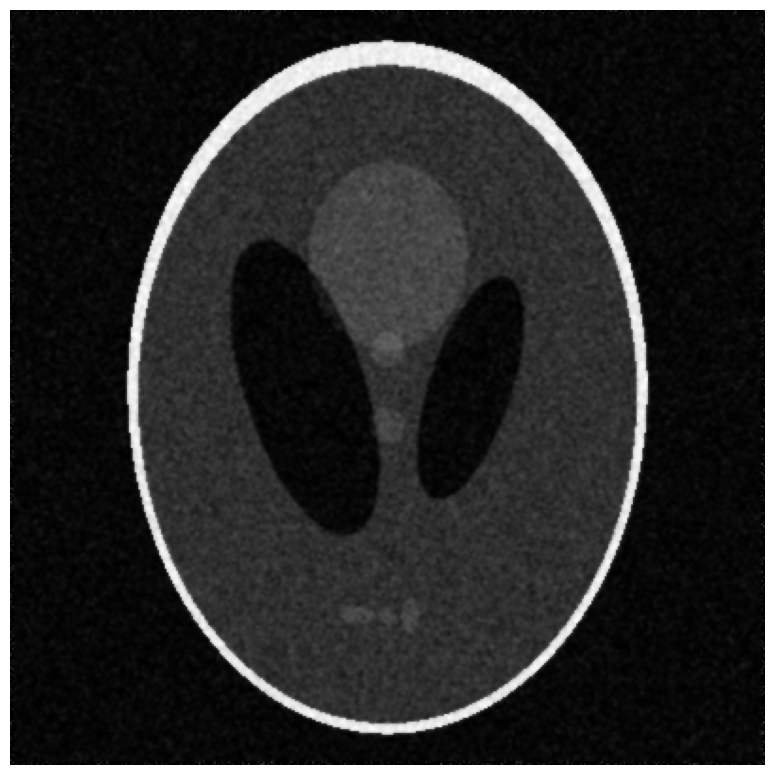
\includegraphics[scale=0.15]{results/anisotropic/image_mse.png}
% \end{columns}
% \end{frame}

\begin{frame}{Data}
\centering
\begin{columns}
\column{.5\textwidth}
\centering
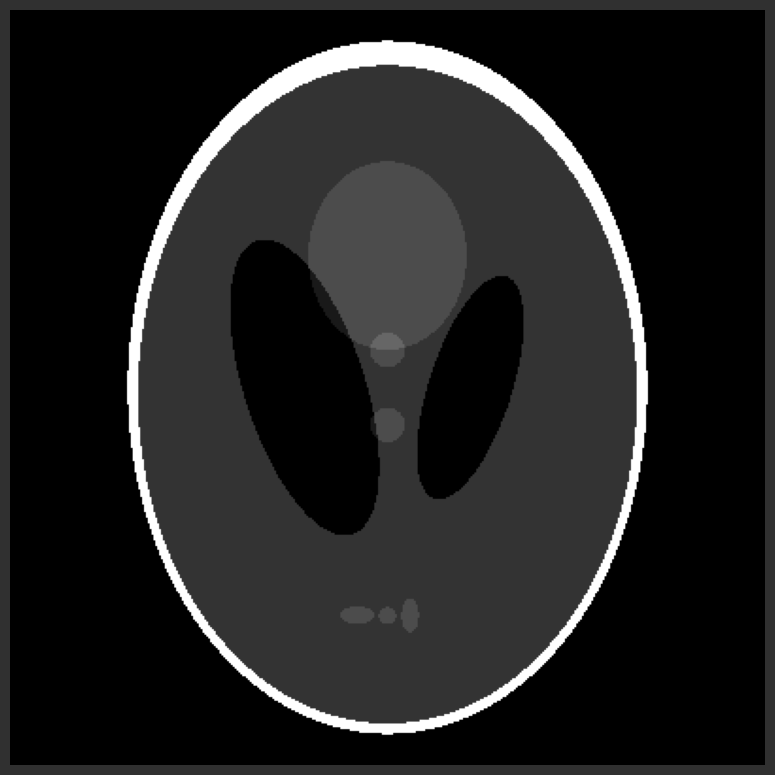
\includegraphics[scale=0.25]{images/results/original.png}
\column{.5\textwidth}
\centering
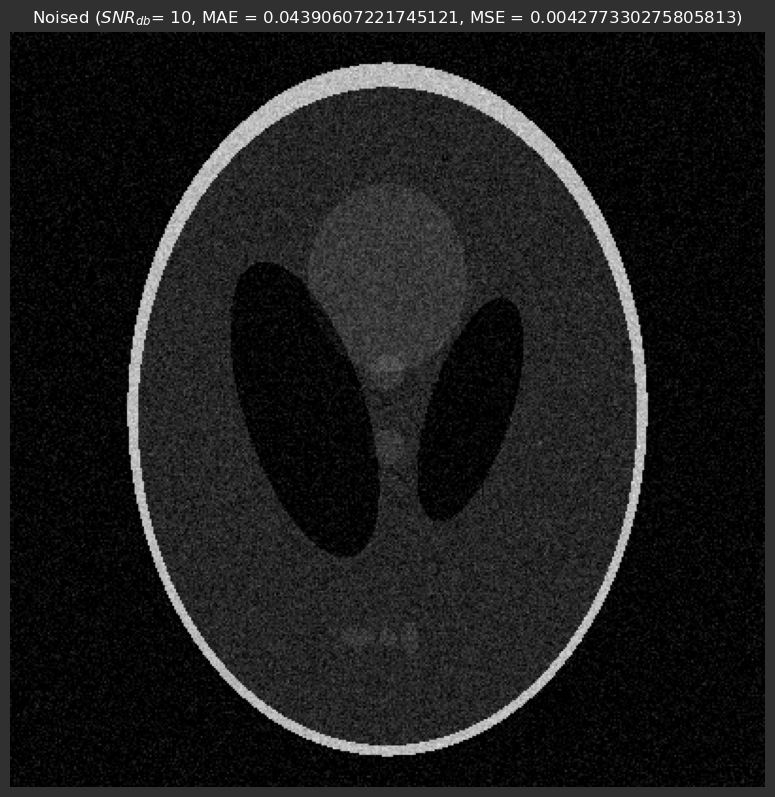
\includegraphics[scale=0.25]{images/results/noised.png}
\end{columns}
\end{frame}

\begin{frame}{Results (with $N = 40$)}
\centering
\begin{columns}
\column{.5\textwidth}
\centering
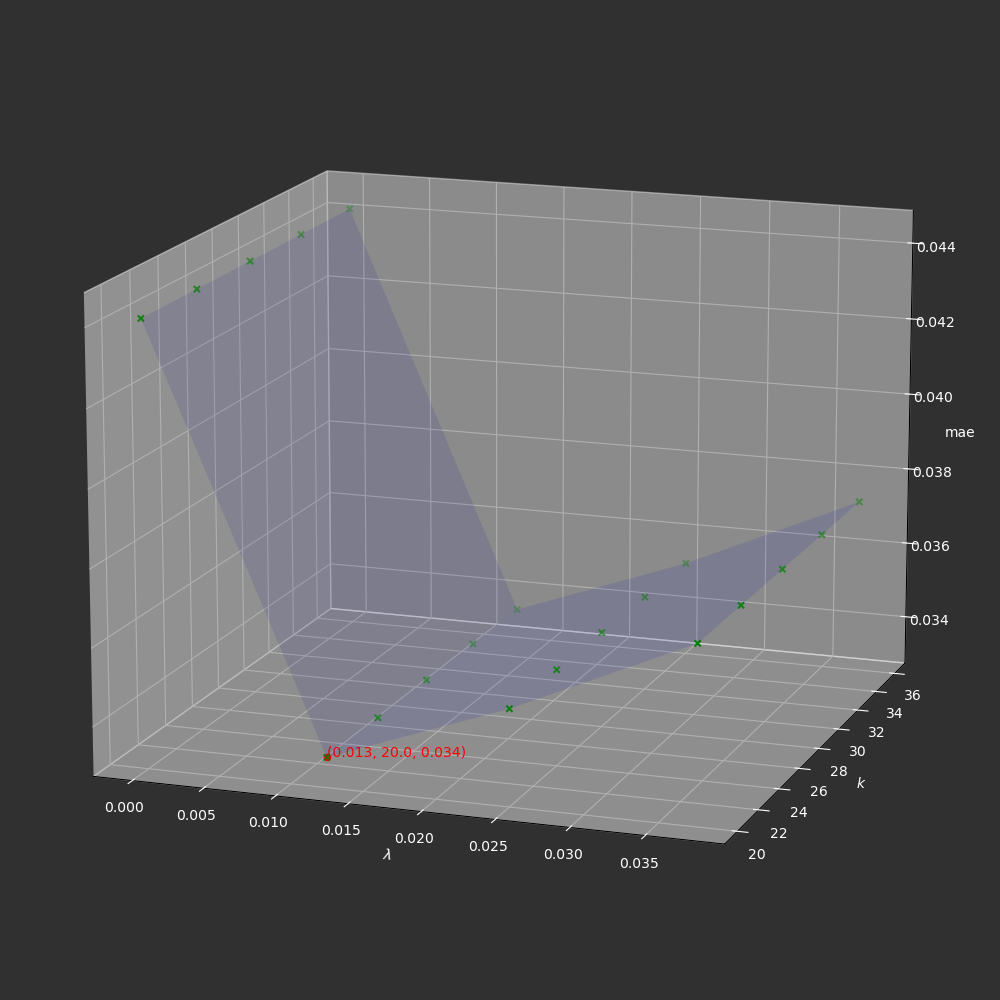
\includegraphics[scale=0.15]{images/results/anisotropic/plot_mae.png}
\column{.5\textwidth}
\centering
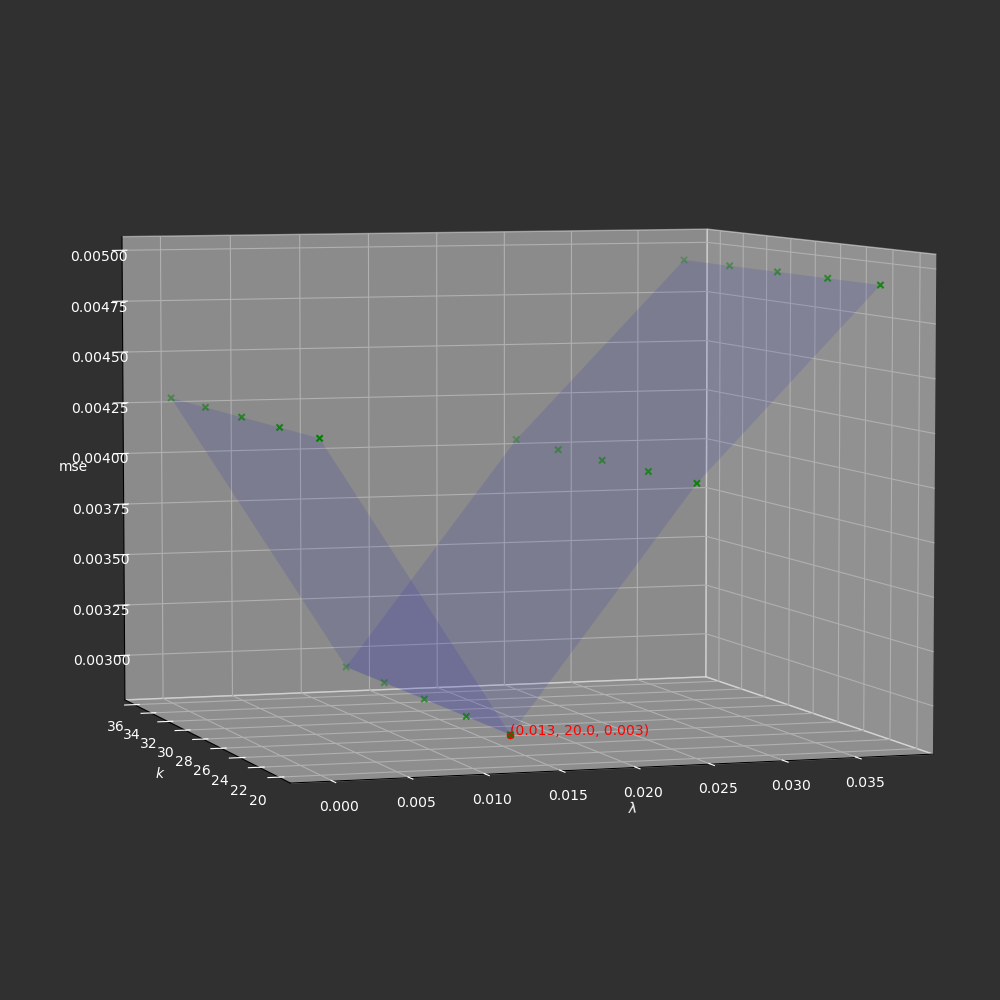
\includegraphics[scale=0.15]{images/results/anisotropic/plot_mse.png}
\end{columns}
\end{frame}

\begin{frame}{Results (with $N = 40$)}
\centering
\begin{columns}
\column{.5\textwidth}
\centering
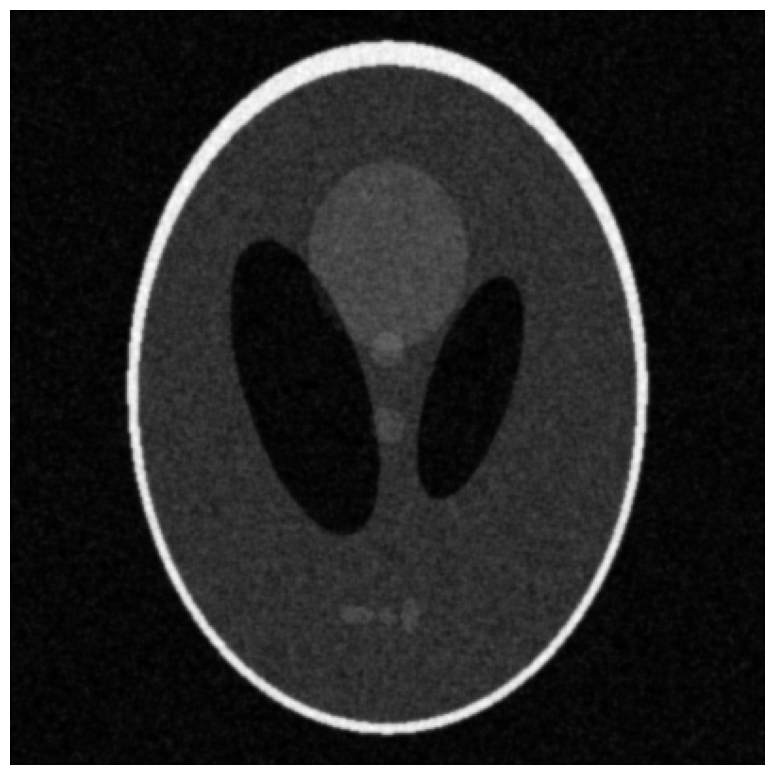
\includegraphics[scale=0.25]{images/results/anisotropic/image_mae.png}
\column{.5\textwidth}
\centering
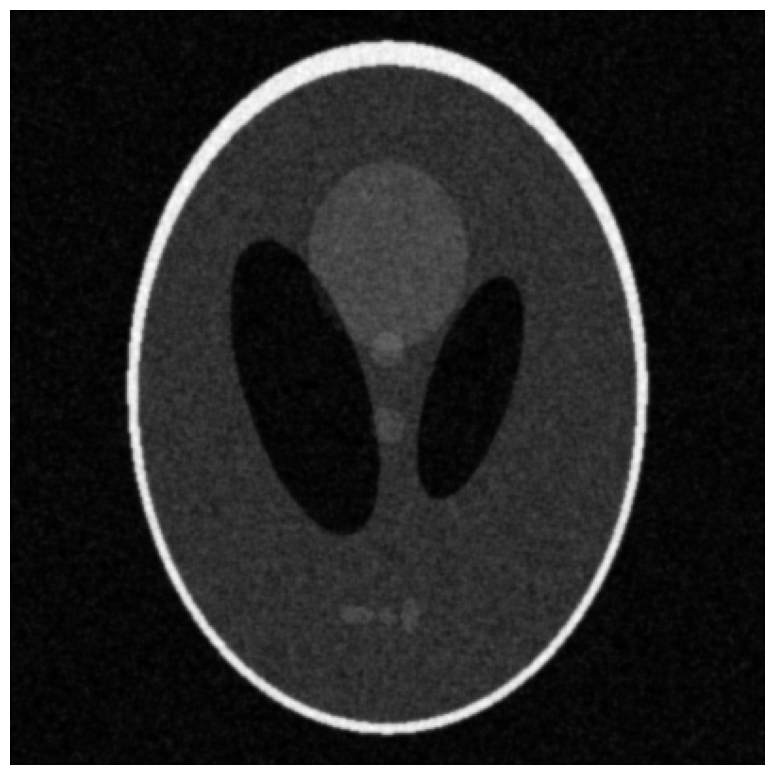
\includegraphics[scale=0.25]{images/results/anisotropic/image_mse.png}
\end{columns}
\end{frame}